\documentclass{bioinfo}
\copyrightyear{2019}
\pubyear{2019}

% \usepackage{hyperref}
\usepackage{url}
\usepackage{amsmath}
\usepackage{array}
\usepackage{booktabs}
\usepackage[normalem]{ulem}
\usepackage{xcolor}
%\usepackage{lmodern}

\usepackage{xspace}
\def\etal{{\em et al.}\xspace}

\usepackage{listings}
\usepackage{color}

\definecolor{dkgreen}{rgb}{0,0.6,0}
\definecolor{gray}{rgb}{0.5,0.5,0.5}
\definecolor{mauve}{rgb}{0.58,0,0.82}

\lstset{
  frame=none,
  % frame=tb,
  numbers=none, % left
  language=Python,
  aboveskip=1mm,
  belowskip=1mm,
  showstringspaces=false,
  columns=flexible,
  basicstyle={\small\ttfamily},
  numberstyle=\tiny\color{gray},
  keywordstyle=\color{blue},
  commentstyle=\color{dkgreen},
  stringstyle=\color{mauve},
  breaklines=true,
  breakatwhitespace=true,
  tabsize=3
}


\providecommand{\e}[1]{\ensuremath{\times 10^{#1}}}
\setlength{\textfloatsep}{11pt}

\access{Advance Access Publication Date: Day Month Year}
\appnotes{Data and text mining}

% Applications notes: Title page, Short Structured Abstract, Text.
\begin{document}
\firstpage{1}

\subtitle{Data and text mining}

\title[openTSNE: a modular Python library for t-SNE dimensionality reduction and embedding]{openTSNE: a modular Python library for t-SNE dimensionality reduction and embedding}
\author[Poli\v{c}ar \textit{et~al}.]{
  Pavlin G. Poli\v{c}ar\,$^{\text{\sfb 1,}*}$
  Martin Stra\v{z}ar\,$^{\text{\sfb 1}}$
  and
  Bla\v{z} Zupan\,$^{\text{\sfb 1, 2}}$}
\address{
$^{\text{\sf 1}}$Faculty of Computer and Information Science, University of Ljubljana, SI-1000 Ljubljana, Slovenia, \\
$^{\text{\sf 2}}$Department of Molecular and Human Genetics, Baylor College of Medicine, Houston TX 77030, U.S.A.
}

\corresp{$^\ast$To whom correspondence should be addressed.}

\history{Received on N/A; revised on N/A; accepted on N/A}

\editor{Associate Editor: TBA}

\abstract{\textbf{Summary:}
Point-based visualisations of possibly large, multi-dimensional data from molecular biology can showcase the data structure and its clusters. One of the most popular techniques to construct such visualisations is t-distributed stochastic neighbor embedding t-SNE, for which a number of extensions have recently been proposed to address speed and quality of resulting visualisations. We propose openTSNE, a modular Python library that implements core t-SNE algorithm and its extensions. The library is orders of magnitude faster than existing popular implementations, including those from scikit-learn, and implements mapping of new data to existing embedding, which can surprisingle assist in solving batch-effect problems.
\\
\textbf{Availability:} openTSNE is available at \url{https://github.com/pavlin-policar/openTSNE}.\\
\textbf{Contact:} \href{pavlin.policar@fri.uni-lj.si}{pavlin.policar@fri.uni-lj.si}\\
% \textbf{Supplementary information:} Supplementary data are available at \textit{Bioinformatics} online.
}

\maketitle

Abundance of high-dimensional data sets in molecular biology calls for techniques for dimensionality reduction, and in particular for methods that can help in construction of data visualisations. From a plethora of approaches, such as principal component analysis, multidimensional scaling, and uniform manifold approximation and projections~\citep{}, t-distributed stochastic neighbor embedding (t-SNE)~\citep{tsne,review-tsne} received much attention as it can address high volumes of data and reveal clustering structure. For instance, recent prominent reports on single cell gene expression data start with an overview of the cell landscape, where t-SNE embeds high-dimensional expression profiles into two dimensional space~\citep{Macosko2015,Shekhar2016,three}. Fig.~\ref{fig:tsne}.a presents an example of such an embedding.

Despite its utility, t-SNE has lately been criticized for insufficient speed when addressing large data sets, lack of global organization of resulting visualisations, where t-SNE focuses on identifying clusters that are then arbitrarily scattered in the low-dimensional space, and absence of theoretically-founded implementations that would map new data into existing embedding. These shortcomings, however, were recently addressed~\citep{ding2018interpretable,becht2019dimensionality}. \citet{fi_tsne} sped-up the embedding through interpolation-based approximation, reducing the complexity of the algorithm to be only linearly dependent on number of data items. \citet{art_of_using_tsne} proposed several techniques including estimating similarities with mixture of Gaussian kernels to improve global alignment. While no current popular software library supports mapping of new data into reference embedding, \citet{parametric_tsne} proposed a related approach with parametric mapping using neural networks.

We here introduce openTSNE, a comprehensive Python library that implements t-SNE and its recently proposed extensions. The library is compatible with Python data science ecosystem (e.g., {\tt numpy}, {\tt sklearn}, {\tt scanpy}). Its modular design fosters extendibility and ease of experimentation with various setting and changes in the analysis pipeline. For example, embedding in Fig.~\ref{fig:tsne}.b using multiscale similarity kernels is obtained through execution of the following code,

\begin{lstlisting}
adata = anndata.read_h5ad("macosko_2015.h5ad")
affinities = openTSNE.affinity.Multiscale(adata.obsm["pca"], perplexities=[50, 500], metric="cosine")
init = openTSNE.initialization.pca(adata.obsm["pca"])
embedding = TSNEEmbedding(init, affinities)
embedding.optimize(n_iter=250, exaggeration=12, momentum=0.5, inplace=True)
embedding.optimize(n_iter=750, momentum=0.8, inplace=True)
\end{lstlisting}

\noindent where we first read the data, define the affinity model based on two gaussian kernels with varying perplexity, use PCA-based initialization, and run the typical two-stage t-SNE optimization. Notice that the code for the standard t-SNE used for Fig.~\ref{fig:tsne}.a is similar but uses only a single kernel ({\tt perplexities=[30]}).

The proposed library supports is currently the only Python t-SNE implementation that supports adding new samples into constructed embedding. For example, we can reuse the {\tt embedding} constructed above to map new data into existing embedding space,

\begin{lstlisting}
new_data = anndata.read_h5ad("shekhar_2016.h5ad")
adata, new_data = find_shared_genes(adata, new_data)
gene_mask = select_genes(adata.X, n=1000)
embedding.affinities = affinity.PerplexityBasedNN(adata[:, gene_mask].X, perplexity=30, metric="cosine")
new_embedding = embedding.transform(new_data[:, gene_mask].X)
\end{lstlisting}

\noindent to load and prepare the new data, define the affinity model, and obtain new embeddings. openTSNE embedds new data one data instance at the time, withouth changing the reference embedding. A side effect of this procedure is handling of batch effects~\cite{Pavlin2019-DS}, a substantial problem in moelcular biology when dealing with the data from different sources~\cite{batch-effects}. The code for plotting of the data is not shown for brevity, but is, together with other examples, available on openTSNE's GitHub page. 

Pure Python implementation introduces computational overhead: openTSNE is about 25\% slower than FIt-SNE~\citep{fi_tsne}, a recent t-SNE implementation in C++, but it is still orders of magnitude faster than other Python implementations (scikit-learn, MulticoreTSNE; see Benchmarks in openTSNE documentation on GitHub). Pure-Python implementation offers distinct advantages that include integration with Python's rich data science infrastructure and ease of installation through PyPI and conda. openTSNE implements controlled execution (callback-based progress monitoring and control), making it suitable for interactive data exploration environments such as Orange~\cite{scorange}.

\section*{Funding and Acknowledgements}
This work was supported by the Slovenian Research Agency Program Grant P2-0209, and by the BioPharm.SI project supported from Eu- ropean Regional Development Fund and the Slovenian Ministry of Education, Science and Sport. We would like to thank George Linderman and Dmitry Kobak for helpful discussions on extensions of t-SNE.

\bibliographystyle{natbib}
\bibliography{policar.bib}
% \end{document}

% \begin{thebibliography}{}
% \end{thebibliography}

\begin{figure}[htbp]
\centerline{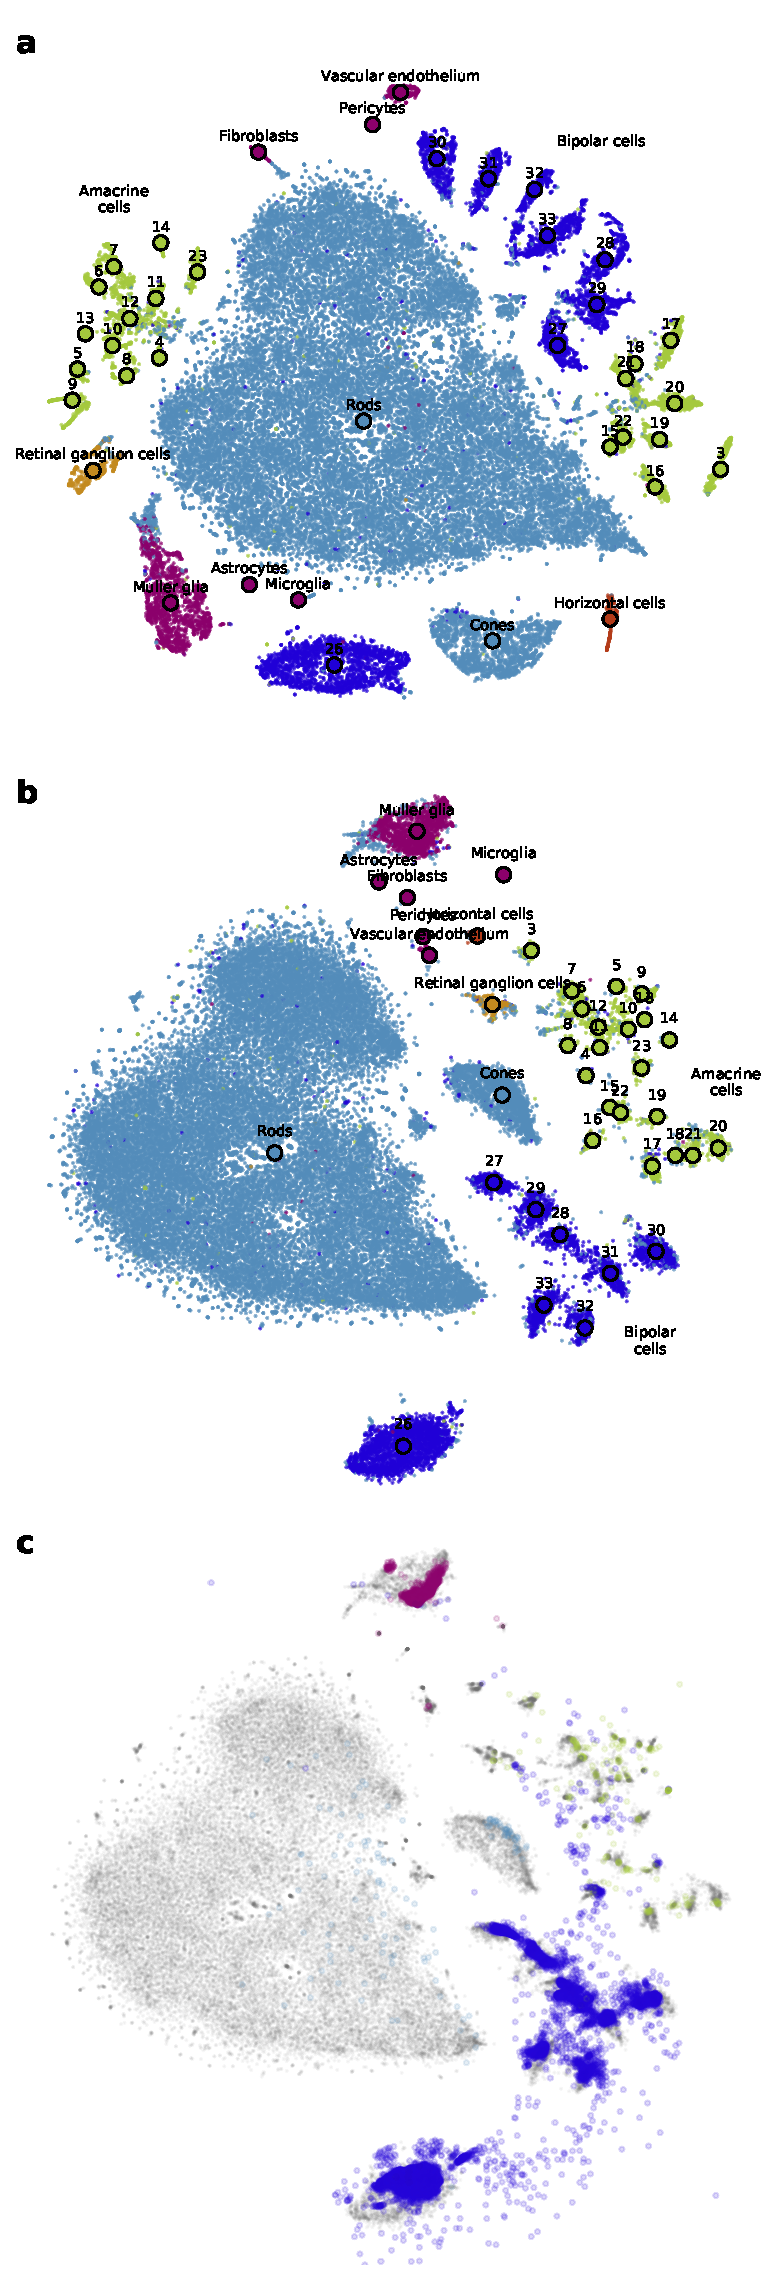
\includegraphics[width=0.7\linewidth]{policar-fig-1}}
\caption{Example of application of openTSNE on single cell data from \citet{Macosko2015} and \citet{Shekhar2016}. a) Standard t-SNE embedding using random initialization and perplexity of 30. b) t-SNE embedding using multi-scale affinities results in better global cluster organization. Cluster annotations in a) and b) are from Macosko~\etal c) Embedding of data from Shekhar~\etal (colored points) on a reference t-SNE visualisation of data from Macosko~\etal (points in gray) places cells in the clusters that match classifications from original publications and alliviates batch effects.}
\label{fig:tsne}
\end{figure}



\end{document}
